
\chapter{Rezultati} % Main chapter title

\label{Rezultati} % For referencing 

Računarska analiza implementirana je u jeziku Pajton \en{Python} verzija 3.6.
Kompletan projekat može se naći na \textit{github} adresi \cite{projekat}. Za
potrebe projekta napravljene su dve baze podataka: relaciona baza podataka
(\textit{PostgreSQL} v9.5) i grafovska baza podataka (\textit{Neo4j} v3.1).

Od 186 MF ključnih reči koje anotiraju bar 20 proteina, 97 je statistički
značajno od čega su 53 predviđeno uređene (p<0.05), a 44 predviđeno neuređene
(p>0.95).  Od 1781 MF termina sa preko 20 pridruženih proteina (dobijeno
grupisanjem, Potpoglavnje \ref{grupisanje}), 1315 je statistički značajno od
čega su 699 predviđeno uređeni, a 616 predviđeno neuređeni.  Tabela
\ref{tab:kw_uopsteno} prikazuje razlike u odnosu na originalne rezultate.

\begin{table}[htpb]
\begin{tabular}{|r|c|c|c|}
  \hline
                     & \small originalni rezultati  & \multicolumn{2}{c|}{ novi rezultati} \\
                     & Xie2007 kw & MF kw  & MF termini                  \\
  \hline
  ukupno ($br. prot\ge20$)     & 143        & 186    & 1781                        \\
  p<0.05 (uređene)   & 37         & 53     & 699                         \\
  p>0.95 (neuređene) & 51         & 44     & 616                         \\
  \hline
\end{tabular}
  \centering
  \caption{Uopšteno poređenje rezultata}
  \label{tab:kw_uopsteno}
\end{table}

Slika \ref{fig:disorder_cmp} sadrži tri tabele predviđeno neuređenih funkcija
koje sadrže: rezultate iz originalnog rada \cite{Xie2007} (levo), nove
rezultate za MF ključne reči (sredina) i rezultate za mapirane MF termine
(desno). Sve tabele su sortirane po z-skoru opadajuće (statistička značajnost
predviđene neuređenosti opada).  Leva tabela sadrži samo 20 statistički
najznačajnije neuređenih MF ključnih reči dok je srednja ograničena na z-skor
veći od dva.  Redovi leve tabele su crveni ako se odgovarajuća ključna reč ne
nalazi u srednjoj tabeli.  Redovi srednje tabele su zeleni ako se nalaze među
prvih 20 a ključna reč se ne javlja u levoj tabeli.  Desna tabela MF termina
sadrži samo one termine koji su rezultat direktnog ili izvedenog mapiranja.
Punim strelicama prikazana su direktna mapiranja, a isprekidanim izvedena.
Nedostatak veze između srednje i desne tabele sugeriše da suprotna funkcija
nije statistički značajna, a crvena boja redova u srednjoj tabeli označava da
ni direktno ni indirektno mapiranje ne postoji.  Srednja i desna tabela pored
kolona z-skor i p vrednosti sadrže i procenat neuređenih proteina
(\text{avg\_dis}) na koji se ubuduće referišemo kao \keyword{neuređenost
funkcije}. Slike \ref{fig:disorder_cmp_ab}a, \ref{fig:disorder_cmp_ab}b
pojednostavljuju sagledavanje pojedinačnih razlika među rezultatima, međutim
zbog ograničenja formata slike neke tabele su skraćene.

Slike \ref{fig:order_cmp} i \ref{fig:order_cmp_ab}  imaju ekvivalentan format
poređenja kao i Slike \ref{fig:disorder_cmp} i \ref{fig:disorder_cmp_ab}, ali
predstavljaju sortirane uređene funkcije.



\clearpage

\begin{figure}[th]
\hspace*{-2.5cm} 
\includegraphics[angle=90, scale=0.45]{Figures/plots/disorder_cmp.pdf}
\decoRule
\caption {
  Poređenje predviđenih neuređenih funkcija
}
\label{fig:disorder_cmp}
\end{figure}

\clearpage

\begin{figure}[th]
\hspace*{-1.0cm} 
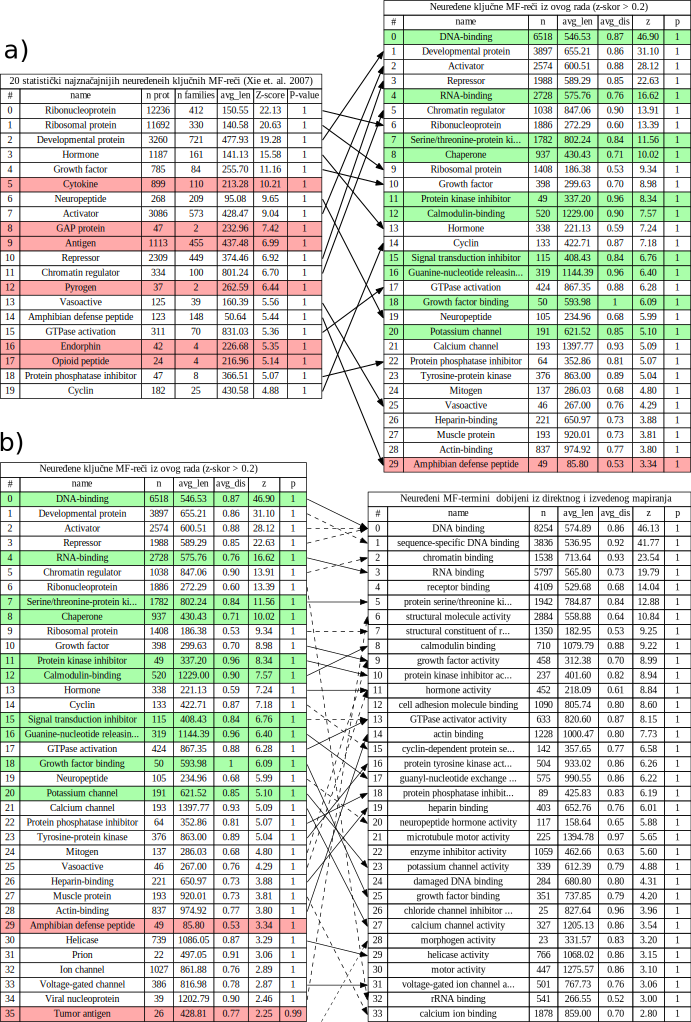
\includegraphics[ scale=0.84]{Figures/plots/disorder_cmp_ab.pdf}
\decoRule
\caption {
  Razdvojeno poređenje predviđenih neuređenih funkcija. Neke tabele su skraćene.
}
\label{fig:disorder_cmp_ab}
\end{figure}

% ------


\begin{figure}[th]
\hspace*{-2.0cm} 
\includegraphics[angle=90, scale=0.45]{Figures/plots/order_cmp.pdf}
\decoRule
\caption {
  Poređenje predviđenih uređenih funkcija
}
\label{fig:order_cmp}
\end{figure}

\begin{figure}[th]
\hspace*{-0.5cm} 
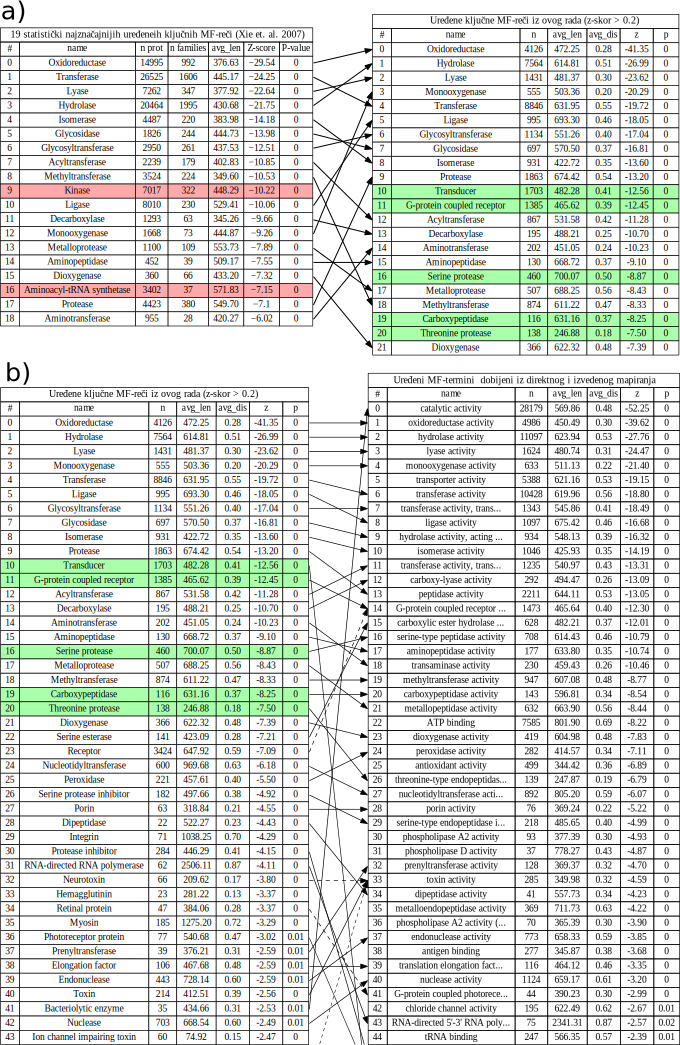
\includegraphics[scale=0.82]{Figures/plots/order_cmp_ab.pdf}
\decoRule
\caption {
  Razdvojeno poređenje predviđenih uređenih funkcija. Neke tabele su skraćene.
}
\label{fig:order_cmp_ab}
\end{figure}


\clearpage

Tabelarni pristup sa Slika \ref{fig:disorder_cmp} i \ref{fig:order_cmp}
prikazuju samo mali podskup svih statistički značajnih MF termina.  Kompletna
analiza grupisanja po MF terminima predstavljena je grafovski, slikama
\file{disorder.svg} i \file{order.svg} koje se nalaze na veb adresi
\cite{rezultati}.  Isečak rezultata \file{disorder.svg} prikazan
je Slikom \ref{fig:disorder_example}.  Pozadinska boja funkcija kodira
\keyword{neuređenost termina}, a kodirana je viridis \cite{viridis} mapiranjem
boja. Viridis mapiranje nulu predstavlja tamno ljubičastom a jedinicu svetlo
žutom pa su tamniji, plavkasti termini  uređeni dok su svetli, zelenkasti
neuređeni.  Rezultujuće \file{.svg} slike su namenjene da budu otvorene u
internet pregledaču.  Držanje kurzora miša iznad funkcija prikazaće dodatne
informacije (ime, definiciju i sinonime), dok će levi klik miša preusmeriti
korisnika na adekvatnu \textit{AmiGO}\footnote{\textit{AmiGO} je skup alat za
pretraživanje i prikazivanje GO termina } ili \uniprot veb stranicu. Desnim
klikom može da se odabere otvaranje stranice u novom tabu pregledača.

\begin{figure}[th]
\hspace*{-2.0cm} 
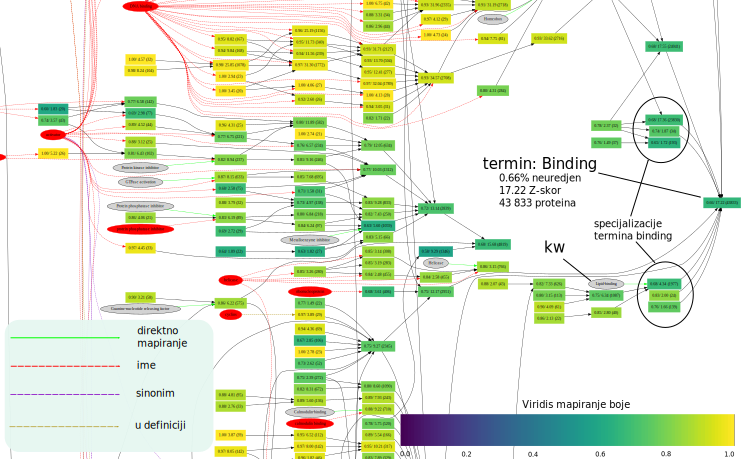
\includegraphics[angle=0, scale=1]{Figures/plots/disorder_example.pdf}
\caption {
  Isečak grafovskog prikaza rezultata (\file{disorder.png}).
}
\label{fig:disorder_example}
\end{figure}


Predloženi $P_L random$ (slučajni) model testirali smo na nivou ključnih reči
izračunavši $z_{rand}$ i  $p_{rand}$ vrednosti za sve MF ključne reči koje
anotiraju bar 20 proteina. Rezultat poređenja z skor vrednosti između $P_L$
modela ($z$-skor) i $P_L random$ modela ($z_{rand}$-skor) prikazan je na Slici
\ref{fig:PLrand}. Prikazane su samo one MF ključne reči koje su statistički
značajne u odnosu na $p$ ili $p_{rand}$ vrednosti dok su crveno obeležene one
ključne reči koje su statistički značajne po jednoj ali ne i drugoj p
vrednosti.


\begin{figure}[th]
\hspace*{-3.0cm} 
\includegraphics[angle=0, scale=1]{Figures/plots/PL_and_PL_rand.pdf}
\caption {
  Poređenje $PL$ i $PL_{random}$ modela nad statistički značajnim predviđenim (ne)uređenim MF ključnim rečima
}
\label{fig:PLrand}
\end{figure}




\chapter{Diskusija} % Main chapter title

\label{Diskusija} % For referencing 

\section{Međusobno upoređivanje MF ključnih reči}

Razmotrimo prvo Sliku \ref{fig:order_cmp_ab}a koja pokazuje da se originalni
rezultati i novi rezultati ne razlikuju bitno za predviđeno uređene MF ključne
reči. Međutim, razlike koje postoje kao i veći izuzeci (\textit{Kinase} i
\textit{Aminoacyl-tRNA synthetase} )  mogu biti posledica drugačijih podataka,
ali i modifikacije metoda originalne analize ili čak kombinacije oba faktora.
Pronalaženje egzaktnog razloga za ove razlike zahteva dodatno istraživanje koje
prevazilazi obim ovog rada.

Sa druge strane, predviđeno \keyword{neuređene} MF ključne reči prikazane na
Slici \ref{fig:disorder_cmp_ab}a imaju znatno više razlika u odnosu na
originalne rezultate.  Šest originalnih MF ključnih reči nije identifikovan u
novim rezultatima. Ipak, \textit{Antigen} u novoj verziji ključnih reči ne
postoji dok su četiri ključne reči izbačene iz analize jer anotiraju ispod 10
CAFA3 proteina (minimum je 20).  Preostala, crvena MF ključna reč
\textit{Cytokine} ima p vrednost 0.49 što je veliko odstupanje od originalnih
rezultat. Značajnu razliku predstavljaju zeleno obeležene MF ključne reči koje
se ne javljaju u originalnim rezultatima, a nalaze se među 20 statistički
najznačajnijih novih rezultata. Među njima \textit{binding} je preovlađujući
motiv što se ne poklapa sa originalnim rezultatima. Za razliku od GO termina,
ključne reči ne sadrže datum dodavanja ili izmene pa ne možemo da proverimo da
li su u pitanju nove ključne reči koje nisu postojale 2006. godine.


\section{Upoređivanje MF ključnih reči i GO termina}

Rezultati prikazni Slikama \ref{fig:disorder_cmp_ab}b i
\ref{fig:order_cmp_ab}b sugerišu značajno poklapanje za statistički
najznačajnije funkcije. Kao što je očekivano, sličnost rezultata $z$-skor i
neurđenost tj.\textit{avg\_dis} pogotovo su izraženi za funkcije koje anotiraju
slične skupove proteina. Veća nepoklapanja prisutna su prvenstveno kod ključnih
reči čije je mapiranje problematično zbog razlika u nomenkulaturi. Na primer
ključna reč \textit{Bacteriolytic enzyme} nalazi se na 42. mestu dok se njen
direktno mapirani MF termin \textit{catalytic activity} nalazi na prvom mestu.

\section{Grafovski prikaz MF termina}

Grafovski prikaz na slikama \file{disorder.svg} i \file{order.svg} predstavlja
odličan medijum za ilustrovanje kompleksnih odnosa između MF termina. Ovaj
prikaz otkriva strukture koje inače ne bi bile uočene.  Opštije MF funkcije
visoke statističke značajnosti okarakterisane su kompleksnom grafovskom
strukturom potomaka. Ipak, ovu strukturu čine isključivo statistički značajni
termini jer bi suprotno rezultat bio  teško saglediv.

\section{Statistička značajnost, neuređenost i broj proteina}

Prosek neuređenih proteina tj. \textit{avg\_dis} (neuređenost) otkriva da
funkcija ne mora da bude pretežno neuređena ili uređena da bi rezultat ($F_J$)
bio statistički značajan.  Na primer, MF termin \textit{hydrolase activity}
(Slika \ref{fig:order_cmp_ab}a) ima $z$-skor $-27.76$, međutim sadrži $53\%$
neuređenih proteina. Ipak prosečna dužina anotiranih proteina je 624, a
verovatnoća da protein te dužine bude klasifikovan kao neuređen je 0.75.
Takođe, veličina skupa anotiranih proteina (11 097 za \textit{hydrolase
activity}) povećava statističku značajnost rezultata. Verovatno je da veliki
broj proteina smanjuje disperziju što vodi ka većim $z$-skor vrednostima.  Ovo
je posebno izraženo kod MF termina \textit{catalytic activity} na Slici
\ref{fig:order_cmp_ab}a.  Iz ovih razloga smatramo da je neophodno uzeti sve
parametre u obzir, a ne samo $z$-skor ili $p$ vrednost.

\section{$P_Lrandom$ model}

Sličnost rezultat $P_L$ i $P_L random$ modela prikazana je na Slici
\ref{fig:PLrand}. Veća odstupanja \\$z_{rand}$-skora kod ključnih reči
\textit{Ribonucleoprotein, Ribosomal protein, Hormone} i drugih ogledaju se
povećanom statističkom značajnošću. Ovo se može objasniti znatno
nižom prosečnom dužinom skupa anotiranih proteina (manje od 300 AK), dok se na
Slici \ref{fig:PL2} uočava da je $P_L random$ verovatnoća niža za proteine
kraće od 300 AK.  Obrnuto, uređene MF ključne reči globalno imaju niži
$z_{rand}$-skor (veću statističku značajnost) što se takođe može objasniti
kombinacijom globalno veće prosečne dužine proteina i većom $P_L random$
verovatnoćom (Slika \ref{fig:PL2}). 

MF ključna reč \textit{Kinase} predstavlja zanimljivo odstupanje jer $P_L
random$ model predviđa statistički značajnu uređenost iako je prosek neuređenih
proteina 0.71 i $P_L$ model predviđa neuređenost. Takođe, MF termin $Kinase
activity$ je statistički značajno neuređena ($P_L$ model).

\section{Klasifikacija neuređenog proteina}

Definicija \ref{pdis_def} neuređenosti proteina iz Potpoglavlja
\ref{naredno} nije uvek idealna.  Na primer, ako je dužina proteina 35 AK, a
neuređenost je predviđena celom dužinom, onda jasno da nema potrebe eliminisati
protein iz analize već ga treba svrstati kao neuređeni.  Takođe, ako je protein
dug 50 AK i sadrži predviđeni neuređeni region od 35 AK, onda treba
pretpostaviti da neuređenost igra ulogu u funkciji. Ovi granični slučajevi čine
suviše mali procenat proteina u CAFA3 podksupu pa je opravdano zanemariti ih.
Međutim, procentualno \swissprot sadrži značajno više kratkih proteina što nas
navodi da istaknemo ovaj problem.

\section{Nastavak istraživanja}

Razvoj novih meta prediktora neuređenosti \cite{mengc2017} svakako je razlog za
nastavak istraživanja. Testiranje novih metoda analize, korišćenje drugih,
većih skupova podataka i novih meta prediktora rezultiraće sigurno interesantnim
rezultatima. Prikaz tih rezultat treba da uključi razvoj korisničkog interfejsa
koji omogućuje interaktivno istraživanje, poređenje i povezanost sa drugim
resursima. Vizuelna komparacija različitih rezultata u grafovskom obliku samo
je jedan od problema koje treba rešiti.

Računarsko istraživanje veze između funkcije i tipa neuređenosti je naredni
pravac koji treba istražiti. Ipak, prediktori koji predviđaju tip neuređenosti
koliko nam je poznato još ne postoje. Iz tog razloga buduće istraživanje treba
da bude fokusirano na njihov razvoj.

